\documentclass[11pt, oneside]{article} 
\usepackage{geometry}
\geometry{letterpaper} 
\usepackage{graphicx}
	
\usepackage{amssymb}
\usepackage{amsmath}
\usepackage{parskip}
\usepackage{color}
\usepackage{hyperref}

\graphicspath{{/Users/telliott_admin/Tex/png/}}
% \begin{center} 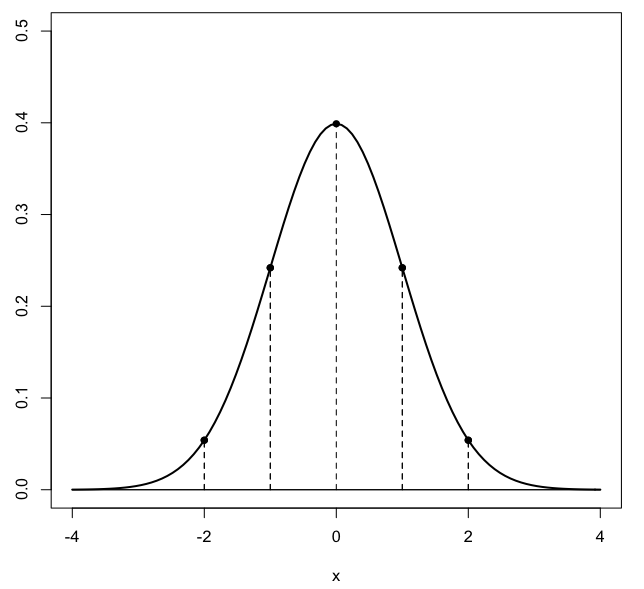
\includegraphics [scale=0.4] {gauss3.png} \end{center}

\title{Numbers}
\date{}

\begin{document}
\maketitle
\Large
Our ideas about sets of numbers start with the counting numbers or positive integers
\[ \mathbb{N} = 1, 2, 3 \dots \]
which is an infinite set.  

Proof by contradiction:  assume there is a greatest natural number.  Add $1$ to it.  $\square$

We extend $\mathbb{N}$ by adding the number or additive identity $0$, plus the negatives of all the numbers in $\mathbb{N}$:
\[ \mathbb{Z} = \{ \dots - 3, -2, -1 , 0 , 1, 2, 3 \dots \} \]

$\mathbb{Z}$ is what they call a \emph{ring}.  The standard operations like addition and multiplication are defined and allowed but not division. 

Then we say, we want division.  We get
\[ \mathbb{Q} = \frac{p}{q}, \ \ \ \  p \in \mathbb{Z}, q \in \mathbb{N} \]

Now, the rational numbers $\mathbb{Q}$ have great properties.  In particular, for any two rational numbers one can find another such number which lies between them:
\[ r = \frac{1}{2} \ [ \ \frac{p_1}{q_1} +  \frac{p_2}{q_2} \ ] \]
This is a rational number and it lies between the two numbers we started with.

\[ \frac{1}{2} \ [ \ \frac{p_1}{q_1} +  \frac{p_1}{q_1} \ ] \ < r < \ \frac{1}{2} \ [ \ \frac{p_2}{q_2} +  \frac{p_2}{q_2} \ ] \]

So it is not unreasonable to have the idea that the number line can be divided into pieces as small as you like by finding rational numbers between rational numbers between rational numbers, and so on.

It sounds good, but there is a big problem:  some numbers cannot be expressed as the ratio of two integers.  For example:  $\sqrt{2}$, $\sqrt{3}$, $\sqrt{5}$, $\sqrt{7}$, etc..  And don't forget $\pi$ and $e$.

The numbers like $\sqrt{2}$ are said to be \emph{irrational} numbers and the set of these, plus all the other numbers is called the real numbers.

This lead Dedekind to formulate the famous Dedekind cut.  Visualize the standard number line as an infinite line on a piece of paper.  

\begin{center} 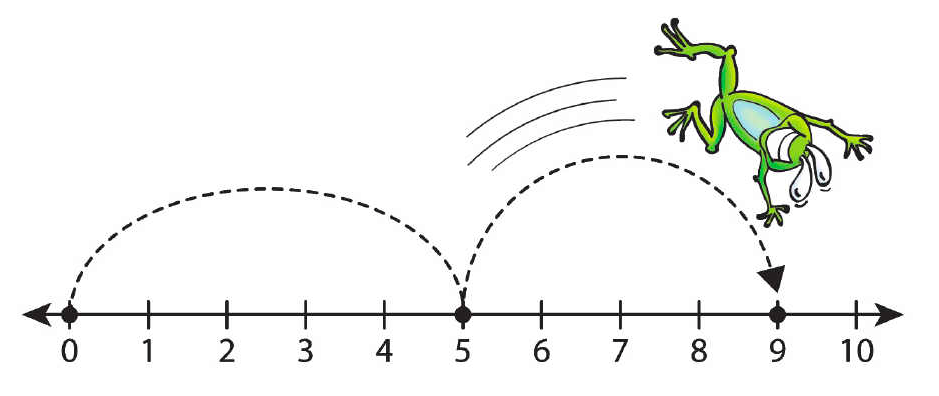
\includegraphics [scale=0.4] {number_line.png} \end{center}

Each real number corresponds to a cut, a knife-edge coming down on this number line.  Every other number is either $>$ or $<$ the number specified by the cut.

One position is $\sqrt{2}$, one is $7/4$ and so on.

It can be shown relatively easily that

• for any two rational numbers one can find a real number which lies between them
• for any two real one can find a rational number which lies between them
• for any two real numbers one can find a real number which lies between them

In other words there is \emph{no largest number} $x$ such that $x < 1$, for example.

That is actually OK.  I can live with what we've said so far.  Here's what's really weird.  Cantor proved that the set $\mathbb{Q}$ is \emph{countably finite}.  Each element in $\mathbb{Q}$ can be paired in order with a member of $\mathbb{N}$.

But the real numbers, $\mathbb{R}$, are countably infinite.  So in some sense, there are many, many, many more irrational numbers than rational numbers.

So when we say that the set of numbers $r < 1$ has \emph{no greatest element}, our problem is two-fold.  We can pick a large rational member of $r < 1$, but we can always find a larger rational element.  

And once we get really close with the large rational element, there are infiinitely more irrational than rational ones waiting beyond.  And yet, given any such very close irrational number, we can always find a larger rational number less than the bound.

I told you it was weird.

\subsection*{e is irrational}

I found a nice proof of the irrationality of $e$ in the calculus text by Courant and Robbins.  It is a proof by contradiction.  We start by assuming that $e$ is rational.
\[ e = \frac{p}{q}, \ \  p,q \in \mathbb{N} \]
We make use of the infinite series representation of $e$
\[ e = 1 + 1 + \frac{1}{2!}  + \frac{1}{3!} + \frac{1}{4!} + \cdots \]
From this, it is obvious that $e > 2$.  If you're interested, there is a proof that $e < 3$ in the book.  

% But I will just say that if $e=p/q$ with $p$ and $q$ integers, and $e>2$, then $q>1$ so $q>=2$.
Equating the series representation to the rational fraction $p/q$:
\[ \frac{p}{q} = 1 + 1 + \frac{1}{2!}  + \frac{1}{3!} + \frac{1}{4!} + \cdots \]
Multiply both sides by $q!$.  For the left-hand side, we have 
\[ e \ q! = \frac{p}{q} \ q! = p (q-1)! \]
We won't need to do anything more with this, but note that since $e\ q!$ is equal to $p (q-1)!$, we can see that the left-hand side, $e\ q!$, is clearly an integer.
Therefore, the right-hand side must also be an integer.  This is the series
\[ q! + q! + \frac{q!}{2!}  + \frac{q!}{3!}  + \cdots + \frac{q!}{(q-1)!} + \frac{q!}{q!} + \frac{q!}{(q+1)!} + \cdots \]
Now, 
$q!$ is obviously an integer. And for every integer $k < q$, $k!$ divides $q!$ evenly 
\[ \frac{q!}{k!} = q \times (q-1) \times (q-2) \cdots \times (q-k+1) \]
In our series
\[ q! + q! + \frac{q!}{2!}  + \frac{q!}{3!}  + \cdots + \frac{q!}{(q-1)!} + \frac{q!}{q!} + \frac{q!}{(q+1)!} + \cdots \]
all the terms to the left of $q!/(q-1)!$ are integers, as is $q!/(q-1)! = q$ and $q!/q! = 1$.  
\vspace{2 mm}

So now our concern is with the fractions that follow.  We will show that these sum up to something less than $1$.  We have
\[ \frac{1}{(q+1)} + \frac{1}{(q+1)(q+2)} + \frac{1}{(q+1)(q+2)(q+3)} + \cdots \]
Since $q >= 2$
\[ \frac{1}{(q+1)} <= \frac{1}{3} \]
\[ \frac{1}{(q+1)(q+2)} <= (\frac{1}{3})^2 \]
and so on, and the entire remaining series of fractions is less than or equal to
\[ \frac{1}{3} + (\frac{1}{3})^2 + (\frac{1}{3})^3 + \cdots \]
This is the geometric series with $r = 1/3$ and first term equal to r, and the sum is known to be
\[ \frac{1}{3} ( 1 / (1-\frac{1}{3}) ) = \frac{1}{2} \]
Since the right-hand side is equal to an integer plus something "less than or equal to $\frac{1}{2}$", it is not an integer, and cannot be equal to the left-hand side, which is equal to an integer.  We have reached a contradiction.  Therefore $e$ cannot be equal to $p/q$, for $p,q \in \mathbb{N}$.

\end{document}